\section{Airline dataset}
\label{sec:resAirline}

\subsection{Digital results}
\label{subsec:digitalAirline}

The digital results of the \ac{NN} once trained are very important. They are the results that the analog system will have to reproduce. Furthermore, this part is used to measure the impact of the custom activation function used for training (\cref{sec:af}).

\begin{figure}[H]
  \centering
  \includesvg[width=\linewidth]{datasets/airlineDigital}
  \caption{Graph of the digital predictions for airline dataset. The dotted vertical line shows the limit of the data used for training and the one used for validation.}
  \label{graph:airlineDigital}
\end{figure}

\Cref{graph:airlineDigital} shows the results of the \ac{NN} next to the orinal data. The results are visually very close. The error is quantified using \ac{RMSE} function. All those curves error to each other are measured and displayed in \cref{tab:airlineDigital}.

\begin{table}[H]
  \centering
  \begin{tabular}{|c|c|c|c|}
    \hline
    %\rowcolor{gray}
    \cellcolor[HTML]{808080}\acs{RMSE} & Original data & Classic prediction & Custom activation functions\\
    \hline
    Original data &\cellcolor[HTML]{202020} & $45.24$ & $45.94$\\
    \hline
    Digital output & $45.24$ & \cellcolor[HTML]{202020} & $4.04$\\
    \hline
    Custom activation function & $45.94$ & $4.04$ & \cellcolor[HTML]{202020}\\
    \hline
  \end{tabular}
  \caption{\acp{RMSE} of each curve to the others}
  \label{tab:airlineDigital}
\end{table}

The error between the digital curves with and without the custom activation functions are visually inexistant. The \ac{RMSE} between those curves confirms this low error as it is of only $4.04$ thousands of passengers away. Considering the values at play, this error is negligible.

Those two curves are both very close to the target curve. They have a very similar error rate to this target curve, indeed they're \ac{RMSE} is $45.24$ for the training using the original activation functions, and $45.94$ for the data created with the analog activation function. The difference of error between the two prediction is of about seven hundred passengers, which is very low considering the scale.

Computing the \ac{NN} with or without the analog activation functions doesn't affect the digital prediction of the \ac{NN}. An error difference so low can be due to the initial weights of the \ac{NN}, before it was trained. Furthermore, training the \ac{NN} for a few more epochs would change the errors by enough to make this difference negligible.

\subsection{Subsection B}
\label{subsec:subbsectiona}

\begin{figure}[H]
  \centering
  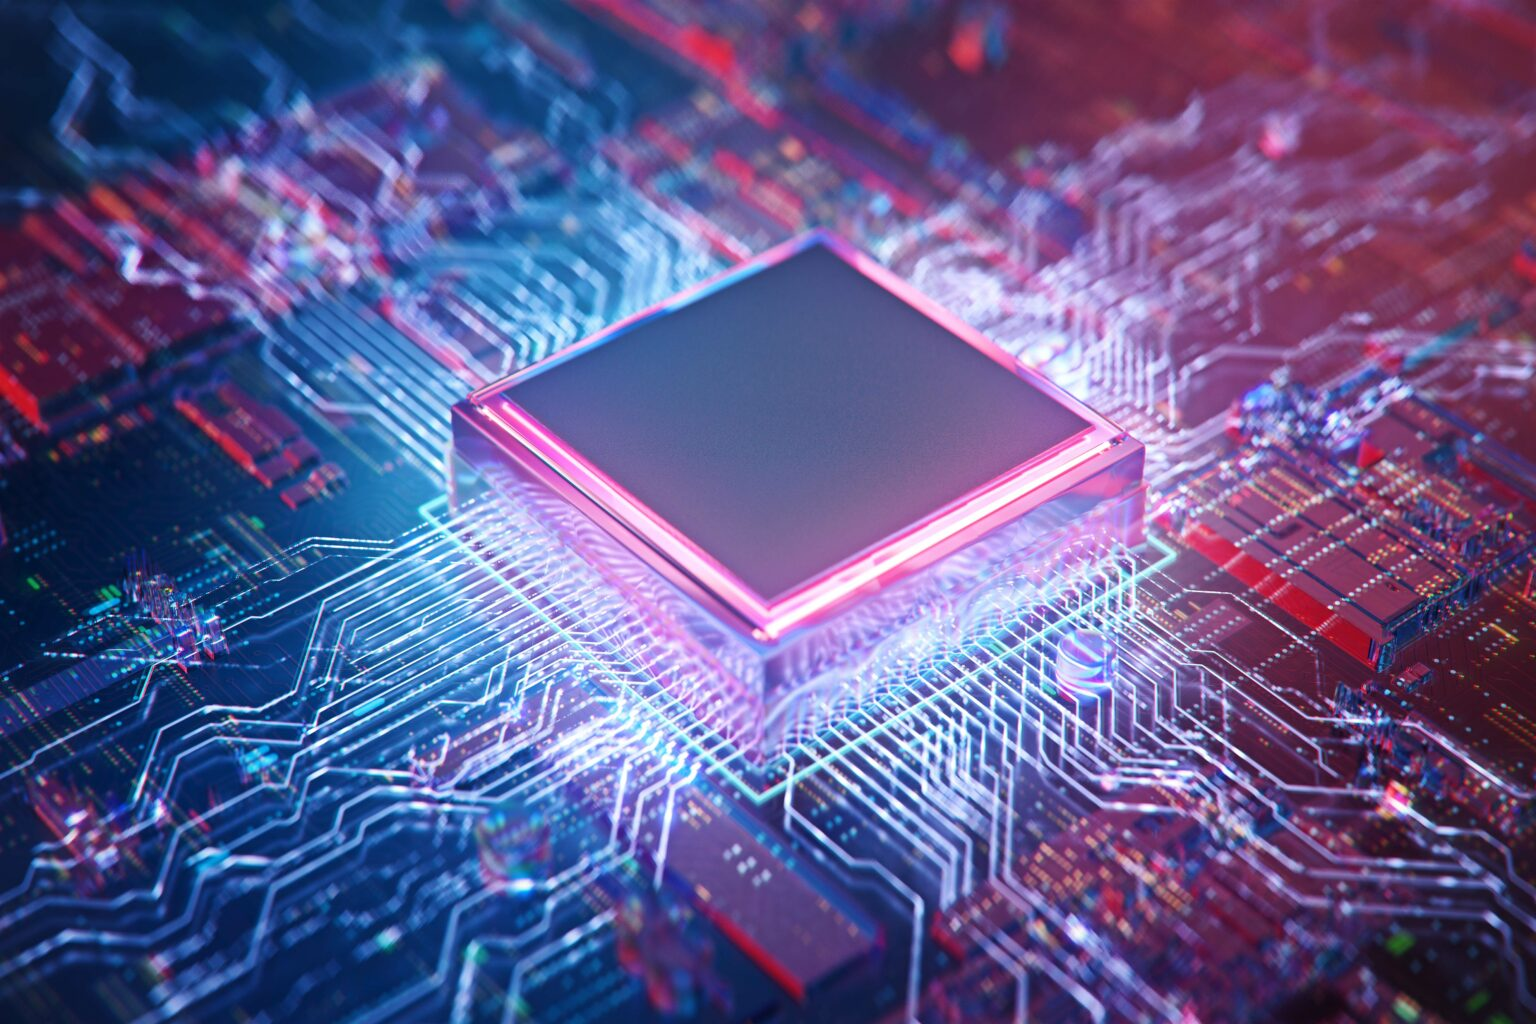
\includegraphics[width=0.5\linewidth]{cover}
  \caption[Dummy Figure Caption for List of Figures.]{Dummy Figure Caption.}
  \label{fig:dummyfigure1}
\end{figure}

Remember you can change the reference style. Another dummy citation \cite{site}.
